
\documentclass[report , a4paper, onecolumn, 12pt]{article}
\usepackage{lscape}
\usepackage{sidecap}
\usepackage{physics}
%\usepackage{bm}
\usepackage{wrapfig}
\usepackage{lipsum}
\usepackage[left=2cm,right=2cm,
    top=2cm,bottom=2cm,bindingoffset=0cm]{geometry}
\usepackage{graphicx}
\usepackage{filecontents}
\usepackage{amsmath}    
\usepackage{amsmath,amsthm,amssymb}
\usepackage{mathtext}
\usepackage[T1,T2A]{fontenc}
\usepackage[utf8]{inputenc}
\usepackage[bulgarian,english,russian]{babel}
\usepackage{braket,mleftright}
\usepackage{enumerate}
\usepackage{enumitem}
\usepackage{graphicx}
\usepackage{caption}
\captionsetup{format =plain}%
\graphicspath{{images/}{../images/}}
\usepackage{blindtext}
\usepackage{hyperref}
\usepackage{listings}
\usepackage{subcaption}
%\renewcommand{\figurename}{Рис.}
%\renewcommand{\tablename}{Табл.}
%\renewcommand*\contentsname{Оглавление}

\usepackage{hyphenat}


\title{Стационарная задача теплопроводности в балке}
\author{Василий Югов, 722 гр.}
\date{Май 2020}
\begin{document}

\maketitle

\tableofcontents

\section{Аннотация}

В работе исследуется применение различных итерационных методов к нахождению решения уравнения Пуассона в квадрате с постоянными граничными условиями первого рода на каждой из сторон. Проводится численное сравнение скорости работы методов Якоби, Зейделя с шахматным и линейным упорядочиванием и метода верхней релаксации с шахматным и линейным упорядочиванием. Также был экспериментально найден порядок сходимости схемы ''крест`` по сетке.

\section{Постановка задачи}

Исследуется классическое двумерное уравнение Пуассона

\begin{equation}
 \pdv[2]{u}{x}(x,y)+\pdv[2]{u}{y}(x,y)=0
\end{equation}

 в прямоугольнике $\Pi = [0, 1] \otimes [0, 1]$ с граничными условиями первого рода

\begin{equation}
 \label{boundary}u(0, y) = 1, \quad u(x, 1) = 2, \quad u(1, y) = 3, \quad u(x, 0) = 4
\end{equation}

Эти уравнения описывают установившееся распределение температур в бесконечно длинной однородной квадратной балке со сторонами, нагретыми до температур 1, 2, 3, 4. Коэффициент теплопроводности балки постоянен. 

Для нахождения решения уравнения Пуассона на сетке будем использовать разностную схему ``крест`` на однородной сетке:

\begin{equation}
 \frac{u_{m - 1, l} - 2 u_{m, l} + u_{m + 1, l}}{h_x^2} + \frac{u_{m,l-1} - 2 u_{m, l} + u_{m, l+1}}{h_y^2} = 0
\end{equation}


Так как задача имеет одинаковый размер вдоль двух направлений, возьмем $h_x = h_y = h = \frac{1}{N - 1}$. Тогда разностное уравнение записывается просто:

\begin{equation}
 \label{cross}u_{m, l} = \frac{1}{4}(u_{m - 1, l} + u_{m + 1, l} + u_{m,l-1} + u_{m, l+1})
\end{equation}

Граничные условия заключаются в задании $u_{m,0}$, $u_{0,l}$, $u_{m, N - 1}$, $u_{N - 1,l}$ в соответствии с \ref{boundary}.

Несложно показать, подставив в \ref{cross} разложение $u$ в ряд Тейлора в окресности узла $(m, l)$, что схема имеет второй порядок аппроксимации. В \cite{aristova} показано, что схема устойчива, т. е. система линейных уравнений \ref{cross} однозначно разрешима, и $||u_{ml}|| \le C ||f||$, где $||f||$ - норма вектора правых частей, т. е. максимум модуля значений на границе. 

Таким образом, все, что осталось - решить систему линейных уравнений \ref{cross}. Делать это будем при помощи итерационных методов: метода Якоби, метода Зейделя и метода верхней релаксации.

\section{Описание исследуемых методов}

Все исследуемые методы являются итерационными, то есть, на каждой итерации следующее приближение решения считается на основе текущего. От метода зависит лишь способ этого пересчета. Будем обозначать верхним индексом номер итерации, нижними - координаты узла.

\subsection{Критерий остановки}

Важен вопрос момента остановки вычислений. Будем пользоваться следующим критерием: на каждой итерации подсчитаем норму разницы текущего приближения и предыдыдущего $e^i = ||u^i - u^{i - 1}||$. Будем считать, что невязки аппроксимируются степенным законом: $\epsilon^i = a k^i$. Тогда можно записать

\begin{equation}
 \epsilon^i = \frac{(e^i)^2}{e^{i - 1} - e^i }
\end{equation}

Когда подсчитанная таким образом величина станет меньше ошибки, к которой мы стремимся, будем останавливать итерации.


\subsection{Исследуемые методы}

\subsubsection{Метод Якоби}

В методе Якоби используется следующая схема:

\begin{equation}
 u^{i + 1}_{ml} = \frac{1}{4} (u^{i}_{m-1, l} + u^{i}_{m, l-1} + u^{i}_{m + 1, l} + u^i_{m, l + 1}) 
\end{equation}

\subsubsection{Метод Зейделя}

Конкретные формулы в методе Зейделя зависят от порядка рассчета узлов. При шахматном упорядочивании сначала считаются узлы с четной суммой индексов, потом узлы с нечетной суммой. Для первых используется формула

\begin{equation}
 u^{i + 1}_{ml} = \frac{1}{4} (u^{i}_{m-1, l} + u^{i}_{m, l-1} + u^{i}_{m + 1, l} + u^i_{m, l + 1}) 
\end{equation}

Вторые считаются на основе уже найденных:

\begin{equation}
 u^{i + 1}_{ml} = \frac{1}{4} (u^{i+1}_{m-1, l} + u^{i+1}_{m, l-1} + u^{i+1}_{m + 1, l} + u^{i+1}_{m, l + 1}) 
\end{equation}

Известно, что одна итерация этого метода эквивалентна двум итерациям метода Якоби \cite{aristova}.

При линейном упорядочивании узлы считаются по порядку(слева направо, снизу вверх) по формуле

\begin{equation}
 u^{i+1}_{ml} =  \frac{1}{4} (u^{i+1}_{m-1, l} + u^{i+1}_{m, l-1} + u^{i}_{m + 1, l} + u^{i}_{m, l + 1}) 
\end{equation}


\subsubsection{Метод верхней релаксации}

Метод является модификацией предыдущего. Он характеризуется параметром $\tau\in (0,2)$, от которого зависит его эффективность. 

При шахматном упорядочивании модифицированная формуля для узлов с четной суммой индексов выглядит как

\begin{equation}
 u^{i + 1}_{ml} = (1-\tau) u^{i}_{m,l} + \tau \frac{1}{4} (u^{i}_{m-1, l} + u^{i}_{m, l-1} + u^{i}_{m + 1, l} + u^i_{m, l - 1}) 
\end{equation}

Узлы с нечетной суммой индексов рассчитываются по формуле

\begin{equation}
 u^{i + 1}_{ml} = (1-\tau) u^{i}_{m,l} + \tau \frac{1}{4} (u^{i + 1}_{m-1, l} + u^{i + 1}_{m, l-1} + u^{i + 1}_{m + 1, l} + u^{i + 1}_{m, l - 1}) 
\end{equation}

Оптимальное значение параметра $\tau$ при таком упорядочении узлов известно \cite{aristova}:

\begin{equation}
\label{tauo}\tau_o = \frac{2}{1 + \sqrt{1 - \rho^2}}
\end{equation}

Здесь $\rho$ - спектральный радиус матрицы перехода метода Якоби. Это соотношение будет в дальнейшем проверено численно.

При линейном упорядочивании модифицированная формула

\begin{equation}
 u^{i+1}_{ml} =  (1-\tau) u^{i}_{m,l}  + \tau \frac{1}{4} (u^{i+1}_{m-1, l} + u^{i+1}_{m, l-1} + u^{i}_{m + 1, l} + u^{i}_{m, l + 1}) 
\end{equation}

\subsection{Теоретическое сравнение скорости сходимости}

Необходимое количество итераций для каждого метода состоит из двух множителей, первый из которых определяется необходимой точностью $ln(\varepsilon)$ \cite{aristova}. Второй множитель различается. Для метода Якоби он равен $\frac{2N^2}{\pi^2}$, для метода Зейделя $\frac{N^2}{\pi^2}$, для метода верхней релаксации при оптимальном выборе параметра $\frac{2N}{\pi}$.

\section{Результаты}

\subsection{Численное решение}

Численное решение было успешно найдено каждым из трех методов. Использовались параметры \hbox{$N = 50, \varepsilon = 10^{-5}$}. 

Карта распределений температур в балке изображена на рис. \ref{fig:heatmap}. Одномерные графики $u(x, y)$ при фиксированных $x$ и $y$ можно увидеть на рис. \ref{fig:profiles}

\begin{figure}[]
    \centering
    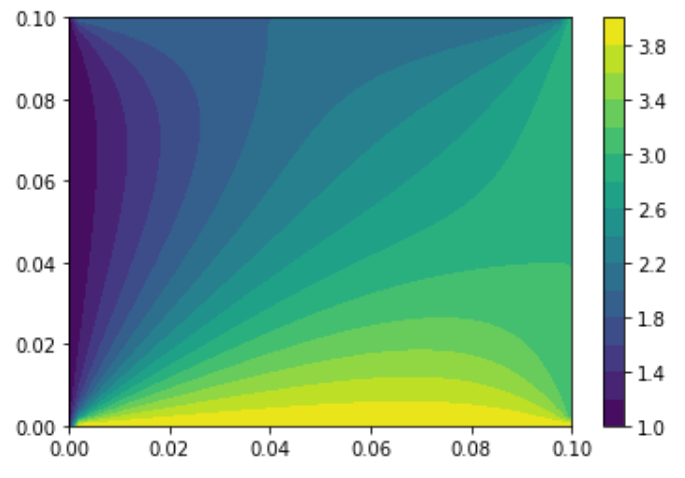
\includegraphics[width=0.6\textwidth]{heatmap}
    \caption{Распределение температур в балке}
    \label{fig:heatmap}
\end{figure}

\begin{figure}[]
    \centering
    \begin{subfigure}{0.5\textwidth}
    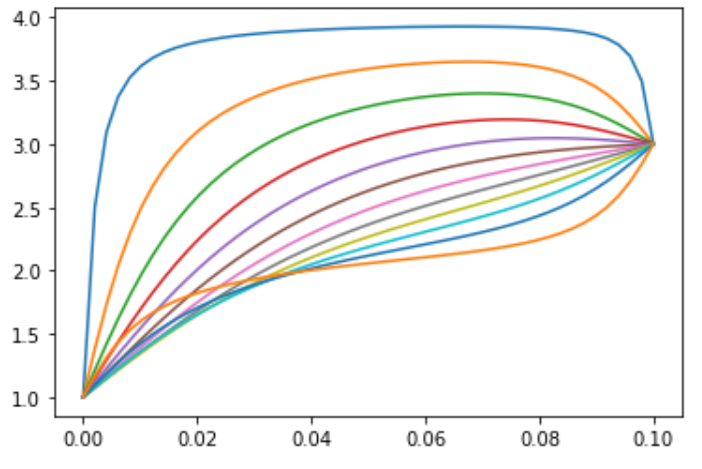
\includegraphics[width=1\textwidth]{profiles_h}
    \caption{На горизонталях $y=\frac{1+4n}{49}$}
    \end{subfigure}%
    \begin{subfigure}{0.5\textwidth}
    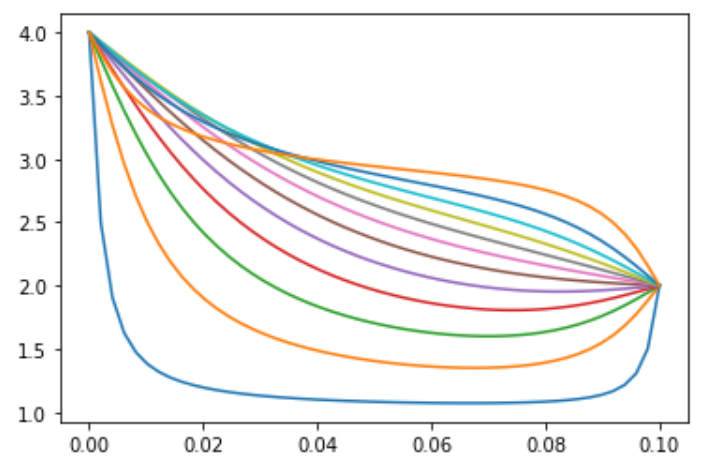
\includegraphics[width=1\textwidth]{profiles_v}
    \caption{На вертикалях $x=\frac{1+4n}{49}$}
    \end{subfigure}
    \caption{Одномерные графики температур}
    \label{fig:profiles}
\end{figure}

\subsection{Численное сравнение скорости сходимости}

Для сравнения скорости сходимости методов будем использовать одинаковые параметры: $N = 50, \varepsilon = 10^{-5}$.

При таких параметрах метод Якоби потребовал $6278$ итераций. Метод Зейделя, независимо от упорядочения, потребовал $3140$ итераций, что почти ровно в два раза меньше. Это объясняется тем, что при таком упорядочении одна итерация метода Зейделя эквивалентна двум итерациям метода Якоби. 

Метод верхней релаксации с шахматным упорядочением исследуем при различных значениях $\tau$ от $\tau = 1.0$ до $\tau = 2.0$ с шагом в $0.01$ и отдельно район минимума с шагом $0.0025$. Изобразим зависимость необходимого числа итераций от $\tau$ на графиках (рис. \ref{fig:taus_chess}).

\begin{figure}[]
    \centering
    \begin{subfigure}{0.5\textwidth}
    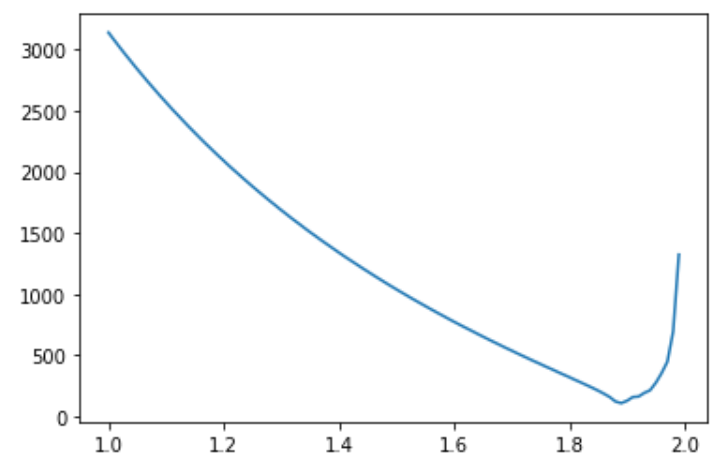
\includegraphics[width=1\textwidth]{taus_chess1}
    \caption{В широком диапазоне}
    \end{subfigure}%
    \begin{subfigure}{0.5\textwidth}
    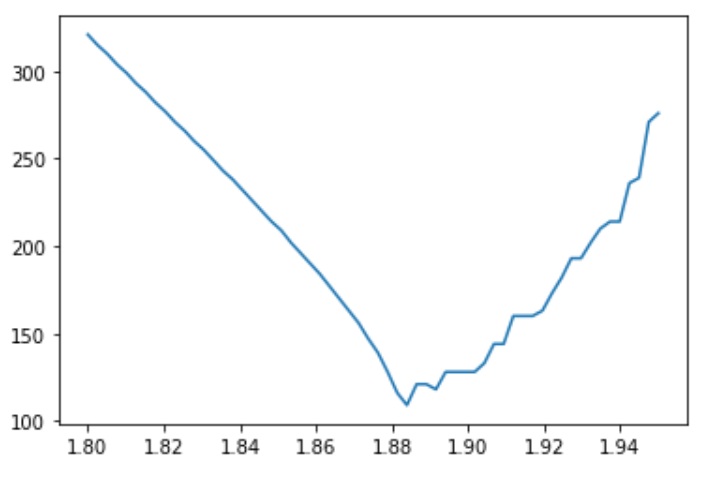
\includegraphics[width=1\textwidth]{taus_chess2}
    \caption{В узком диапазоне}
    \end{subfigure}
    \caption{Зависимость числа итераций метода верхней релаксации с шахматным упорядочением от $\tau$}
    \label{fig:taus_chess}
\end{figure}

Минимум в 109 итераций достигается при $\tau_o = 1.884$. 

Сравним это со значением, предсказываемым формулой \ref{tauo}. Спектральный радиус $\rho$ матрицы перехода метода Якоби найдем при помощи последовательного применения итерации метода Якоби с нулевыми граничными условиями к произвольным образом изначально заданному вектору $u$. После 10000 итераций получился результат $\rho = 0.99795$. Тогда рассчитанное по формуле \ref{tauo} оптимальное значение равно $\tau_o = 1.880$. Видим, что теория хорошо подтвердилась на практике.

Аналогично исследуем метод верхней релаксации  с линейным упорядочнием.  Зависимость числа итераций от параметра $\tau$ изображена на рис. \ref{fig:taus_linear}. Минимум в 129 итераций достигается при $\tau_o=1.884$. Можно сделать вывод, что при значения оптимального параметра $\tau$ для двух упорядочиваний совпадают, но при линейном упорядочивании требуется немного больше итераций, чем при шахматном.

\begin{figure}[]
    \centering
    \begin{subfigure}{0.5\textwidth}
    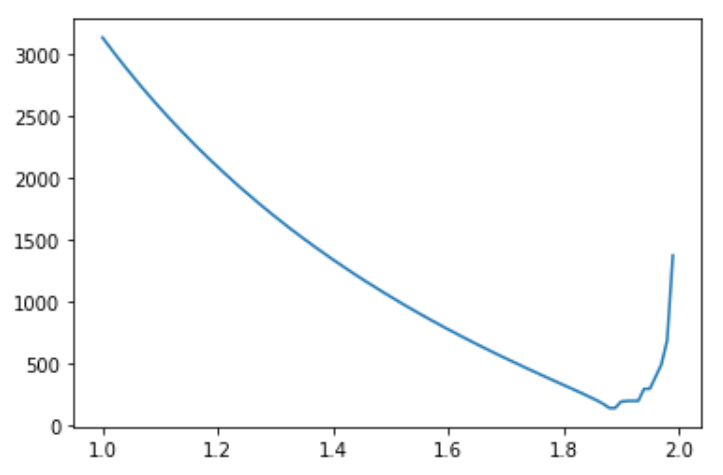
\includegraphics[width=1\textwidth]{taus_linear1}
    \caption{В широком диапазоне}
    \end{subfigure}%
    \begin{subfigure}{0.5\textwidth}
    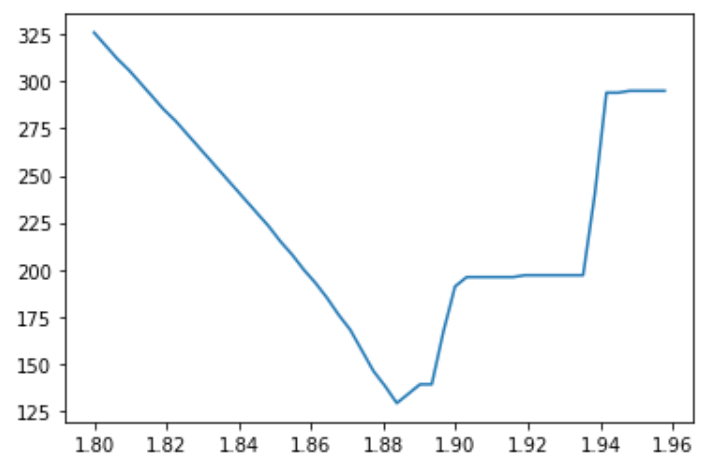
\includegraphics[width=1\textwidth]{taus_linear2}
    \caption{В узком диапазоне}
    \end{subfigure}
    \caption{Зависимость числа итераций метода верхней релаксации с линейным упорядочением от $\tau$}
    \label{fig:taus_linear}
\end{figure}

\subsection{Скорость сходимости по сетке}

Численно оценим скорость сходимости схемы ''крест`` по сетке. Для этого найдем решения $u^{(50)}, u^{(100)}, u^{(200)}$ на сетках  $N_1 = 51$, $N_2 = 101$ и $N_3 = 201$. Найдем для двух самых крупных и двух самых мелких сеток разницы в общих узлах трех сеток.  Найдем $L_1$ нормы этих разностей. Тогда порядок сходимости схему можно рассчитать по формуле $ p^{(e)}=\log_2\left(\frac{||u^{(100)}-u^{(50)}||}{||u^{(200)} - u^{(100)}||}\right)$. Численные результаты равны

\begin{equation}
 ||u^{(100)} - u^{(50)}||_1 = 0.603, \quad  ||u^{(200)} - u^{(100)}||_1 = 0.161, \quad p^{(e)}=\log_2\left(\frac{||u^{(100)}-u^{(50)}||}{||u^{(200)} - u^{(100)}||}\right)=1.91
\end{equation}

Найденный порядок сходимости близок к теоретиески известному $p^{(t)} = 2$.

\section{Вывод}

Таким образом, каждый из итерационных методов оказался пригоден к решению поставленной задачи. Численно найденные скорости работы методов соответствуют теоретическим предсказаниям. Самым быстрым из исследованных методов является метод верхней релаксации с шахматным упорядочиванием. Численно найденный порядок сходимости схемы ''крест`` $p^{(e)}=1.91$ соответствует известному из теории значению $p^{(t)}=2$.


\begin{thebibliography}{9}
\bibitem{aristova} 
Е. Н. Аристова, А. И. Лобанов
\textit{Практические занятия по вычислительной математике в МФТИ. Часть 2.}. 
МФТИ, Москва, 2015

\end{thebibliography}

\end{document}
